\documentclass[uplatex,dvipdfmx]{jsarticle}

\usepackage[fleqn,tbtags]{mathtools}
\usepackage{geometry}
\usepackage{setspace}
\usepackage{tabularx}%\usepackage[uplatex,deluxe]{otf} % UTF
\usepackage{stix2} %欧文＆数式フォント
\usepackage[fleqn,tbtags]{mathtools} % 数式関連 (w/ amsmath)
\usepackage{graphicx}
\usepackage{float}
\usepackage{caption} % キャプションの設定に必要
\usepackage{subcaption} % subfigureに必要
\usepackage{enumitem} % リストのカスタマイズに必要
\usepackage[hyphens]{url} % 先にurlパッケージ読込
\usepackage[hidelinks,dvipdfmx]{hyperref}
\usepackage{amsmath}
\usepackage{ascmac}
\usepackage[uplatex,deluxe]{otf} % UTF
\usepackage[noalphabet]{pxchfon} % must be after otf package
\usepackage{stix2} %欧文＆数式フォント
\usepackage[fleqn,tbtags]{mathtools} % 数式関連 (w/ amsmath)
\usepackage{graphicx}
\usepackage[dvipdfmx]{color}
\usepackage{listings} % パッケージの読み込み
\lstset{
    basicstyle=\ttfamily\small, % 基本フォント
    breaklines=true, % 長い行を自動で折り返す
    frame=single, % コードを枠で囲む
    numbers=left, % 行番号を左に表示
    captionpos=b, % キャプションを下に表示
    xleftmargin=\parindent, % 左マージン
    tabsize=2, % タブのサイズ
}
\usepackage{verbatimbox}
\begin{document}

\title{Webプログラミング Webアプリの表示}
\author{25G1125 松山優翔}
\date{2025年7月21日}
\maketitle

\section{開発者向け}

\subsection{サイゼリヤ メニュー管理システム}

\subsubsection{概要}
サイゼリヤ メニュー管理システムは，飲食店のメニュー情報を管理することを目的としたWebアプリケーションである．注文番号・商品名・ジャンル・税込価格などの情報を一覧で表示し，商品名をクリックすることで詳細画面へ遷移する．また，新規メニューの追加や既存メニューの編集・削除が可能であり，実際の業務用管理画面を意識した設計とした．

\subsubsection{データ構造}
まずここにデータ構造を表1に示す．
idは識別用として用い，codeはサイゼリヤで客自身が注文する際に入力する注文番号，nameはメニュー表に書いてある商品名，categoryは商品のジャンル，priceは税込価格であり，また文字列として保持し表示の簡潔さを優先した．

\begin{table}[H]
    \centering
    \caption{データ構造}
    \label{tab:pulse_comparison}
    \setlength{\extrarowheight}{3pt} 
    \begin{tabular}{|c|c|c|}
        \hline
        キー名 & 型 & 内容 \\
        \hline
        id & Number & 識別用 \\
        \hline
        code & Number & 注文番号 \\
        \hline
        name & String & 商品名 \\
        \hline
        category & String & ジャンル \\
        \hline
        price & String & 税込価格 \\
        \hline
     \end{tabular}
\end{table}

\subsubsection{HTTPメソッドとリソース名一覧}
次にHTTPメソッドとリソース名一覧を表2に示す．
一覧表示ではEJSテンプレートを用いて，登録されている全メニュー情報を表形式で表示する．
この際，商品名を一覧として確認できるようにしている．
詳細表示ではURLパラメータとして受け取った番号を配列のインデックスとして使用し，
該当するメニュー1件の詳細情報（種別を含む）を表示する．
新規追加，編集，更新，削除の各機能を実装することで，
完全なCRUD（Create / Read / Update / Delete）操作を可能としている．

\begin{table}[H]
    \centering
    \caption{HTTPメソッドとリソース名一覧}
    \label{tab:pulse_comparison}
    \setlength{\extrarowheight}{3pt} 
    \begin{tabular}{|c|c|c|}
        \hline
        機能 & メソッド & リソース名 \\
        \hline
        一覧表示 & Get & /saize \\
        \hline
        詳細表示 & Get & /saize/:number \\
        \hline
        追加 & Get & /saize/new \\
        \hline
        追加実行 & Post & /saize/create \\
        \hline
        編集 & Get & /saize/edit/:number \\
        \hline
        更新 & Post & /saize/update/:number \\
        \hline
        削除 & Post & /saize/delete/:number \\
        \hline
     \end{tabular}
\end{table}

\subsubsection{リソース名ごとの機能の詳細}
\textbf{/saize} : 登録されている全メニュー情報を配列から取得し，EJSテンプレートを用いて一覧表示を行う．
閲覧専用の処理であるため GET メソッドを使用している．\\
\textbf{/saize/:number} : URLパラメータで受け取った番号を配列のインデックスとして使用し，該当メニュー1件の詳細情報を表示する．番号に応じて表示内容が変化するため，動的ルーティングを採用している．\\
\textbf{/saize/new} : 新規メニュー登録用の入力フォームを表示する画面である．サーバ側のデータを変更しないため GET メソッドを使用している．\\
\textbf{/saize/create} : フォームから送信された注文番号・商品名・ジャンル・価格を受け取り，新しいオブジェクトとして配列に追加する．データを新規作成する処理のため POST メソッドを使用している．\\
\textbf{/saize/edit/:number} : 指定されたメニューの既存情報をフォームに初期値として表示し，編集可能な状態にする．
表示処理のみであるため GET メソッドを使用している．\\
\textbf{/saize/update/:number} : 編集フォームから送信された内容を用いて，指定番号のデータを上書き更新する．
既存データを変更する処理のため POST メソッドを使用している．\\
\textbf{/saize/delete/:number} : 指定された番号のメニュー情報を配列から削除する．誤操作防止の観点から GET ではなく POST メソッドを使用している．
\subsubsection{遷移図}
ここにサイゼリヤ メニュー管理システムにおいてのデータの遷移図を図1に示す．

\begin{figure}[H]
\begin{center}
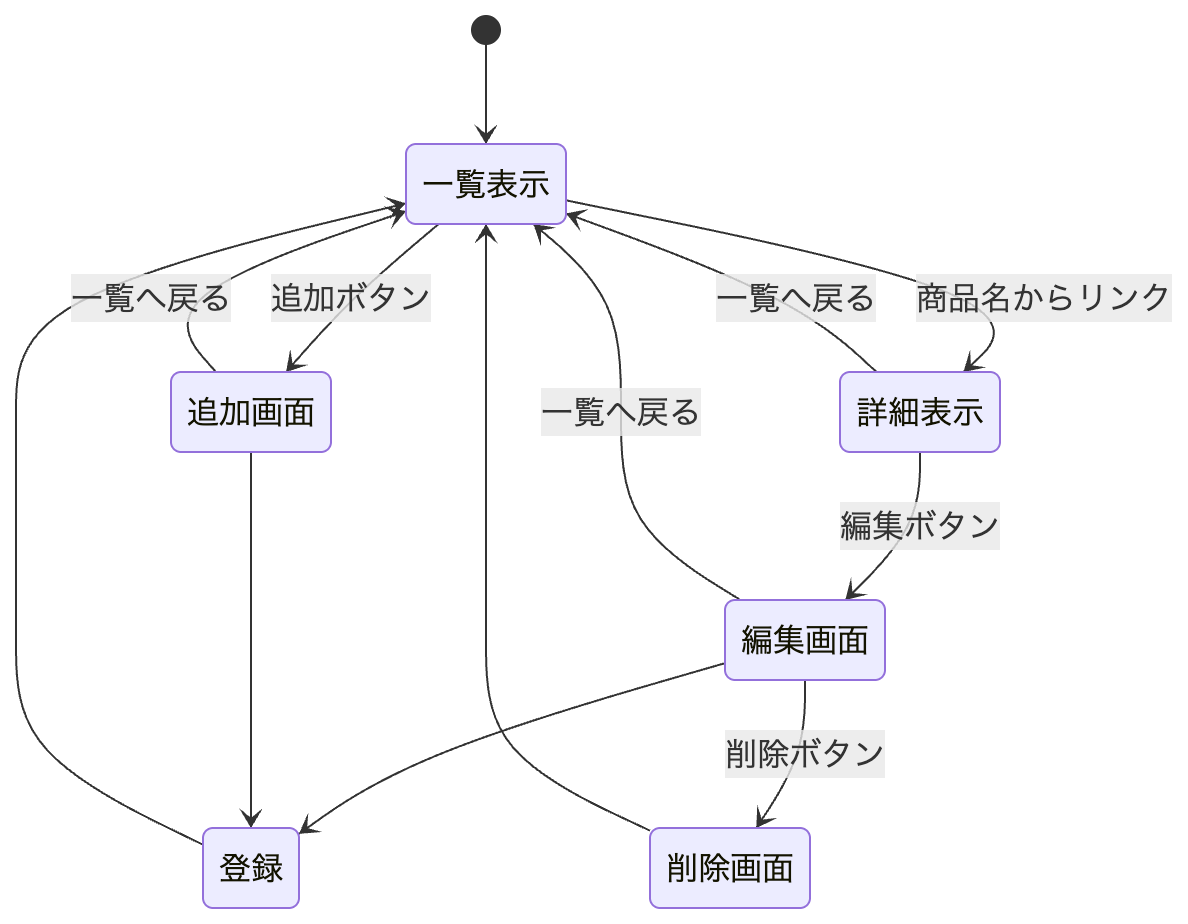
\includegraphics[width=0.5\textwidth,clip]{seni.png}
\end{center}
\caption{\textgt{サイゼリヤ メニュー管理システムの遷移図}}
\label{sample}
\end{figure}

\subsection{Bリーグ チーム管理システム}

\subsubsection{概要}
Bリーグ チーム管理システムは，日本のプロバスケットボールリーグであるBリーグに所属するB1・B2全チームの情報を管理するWebアプリケーションである．単なる一覧表示ではなく，地域やホームアリーナ，主要選手，優勝回数などスポーツチーム特有の多様なデータを扱う点が特徴である．

\subsubsection{データ構造}
まずここにデータ構造を表3に示す．
idは識別用として用い，nameは男子バスケットボールリーグに所属しているチーム名，divisionはB1,B2区分，regionはチームがホームタウンとしてる地域，arenaはチーム会場だけでなくチームの経営などを行うアリーナ，playersはそのチームにおける主要メンバー，championshipsはそのチームの歴代優翔回数，foundedはそのチームの設立年である．

\begin{table}[H]
    \centering
    \caption{データ構造}
    \label{tab:pulse_comparison}
    \setlength{\extrarowheight}{3pt} 
    \begin{tabular}{|c|c|c|}
        \hline
        キー名 & 型 & 内容 \\
        \hline
        id & Number & 識別用 \\
        \hline
        name & String & チーム名 \\
        \hline
        division & String & 区分(B1/B2) \\
        \hline
        region & String & 地域 \\
        \hline
        arena & String & アリーナ \\
        \hline
        players & String & 主要メンバー \\
        \hline
        championships & Number & 優勝回数 \\
 	\hline
        founded & Number & 設立年 \\
        \hline
     \end{tabular}
\end{table}

\subsubsection{HTTPメソッドとリソース名一覧}
次にHTTPメソッドとリソース名一覧を表4に示す．
一覧表示ではEJSテンプレートを用いて，登録されている全チーム情報を表形式で表示する．
この際，チーム名を一覧として確認できるようにしている．
詳細表示ではURLパラメータとして受け取った番号を配列のインデックスとして使用し，
該当するチーム1件の詳細情報（種別を含む）を表示する．
新規追加，編集，更新，削除の各機能を実装することで，
完全なCRUD（Create / Read / Update / Delete）操作を可能としている．
\begin{table}[H]
    \centering
    \caption{HTTPメソッドとリソース名一覧}
    \label{tab:pulse_comparison}
    \setlength{\extrarowheight}{3pt} 
    \begin{tabular}{|c|c|c|}
        \hline
        機能 & メソッド & リソース名 \\
        \hline
        一覧表示 & Get & /bleague \\
        \hline
        詳細表示 & Get & /bleague/:number \\
        \hline
        追加 & Get & /bleague/new \\
        \hline
        追加実行 & Post & /bleague/create \\
        \hline
        編集 & Get & /bleague/edit/:number \\
        \hline
        更新 & Post & /bleague/update/:number \\
        \hline
        削除 & Post & /bleague/delete/:number \\
        \hline
     \end{tabular}
\end{table}

\subsubsection{リソース名ごとの機能の詳細}
\textbf{/bleague} : Bリーグに所属するB1・B2全チームの情報を配列から取得し，一覧表示する．チーム名をクリックすることで詳細画面へ遷移できる．\\
\textbf{/bleague/:number} : URLパラメータで指定された番号のチーム情報を表示する．地域・アリーナ・主要メンバー・優勝回数・設立年など，スポーツチーム特有の詳細情報を確認できる．\\
\textbf{/bleague/new} : 新規チーム情報を登録するための入力フォームを表示する画面である．．\\
\textbf{/bleague/create} : フォームから送信されたチーム情報を受け取り，新しいチームデータとして配列に追加する．\\
\textbf{/bleague/edit/:number} : 既存チーム情報をフォームに初期値として表示し，編集可能な状態にする．\\
\textbf{/bleague/update/:number} : 編集後の内容で指定されたチームデータを上書き更新する．\\
\textbf{/bleague/delete/:number} : 指定されたチーム情報を配列から削除する．データ消去という重要操作のため POST メソッドを使用している．
\subsubsection{遷移図}
ここにBリーグ チーム管理システムにおいてのデータの遷移図を図2に示す．

\begin{figure}[H]
\begin{center}
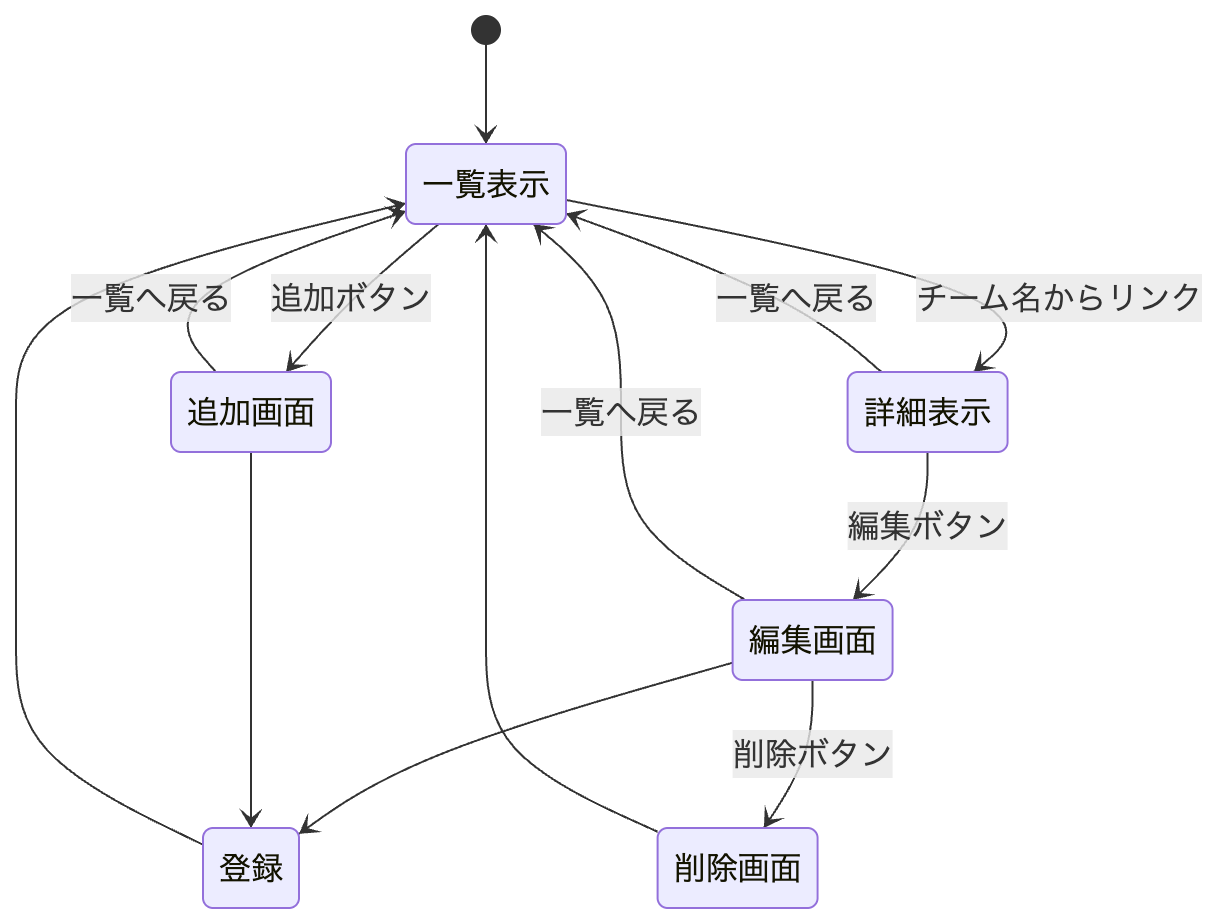
\includegraphics[width=0.5\textwidth,clip]{senii.png}
\end{center}
\caption{\textgt{Bリーグ チーム管理システムの遷移図}}
\label{sample}
\end{figure}

\subsection{ヤングスキニー アルバム管理システム}

\subsubsection{概要}
ヤングスキニー アルバム管理システムは，日本のロックバンド「ヤングスキニー」が発表したフルアルバムおよびEP作品の情報を管理することを目的としたWebアプリケーションである．アルバム名，発売年，所属レーベル，アルバム種別（フルアルバム／EP），収録曲，初回限定版DVDの収録内容といった音楽作品特有の詳細な情報を扱う点が特徴である．一覧画面ではアルバム名，発売年を確認でき，アルバム名をクリックすることで詳細画面へ遷移する．また，新規アルバムの追加，既存データの編集および削除が可能であり，アーティスト作品のデータベース管理を想定した構成とした．

\subsubsection{データ構造}
まずここにデータ構造を表5に示す．
idは識別用として用い，titleはヤングスキニーのインディーズ作品からメジャー作品までのアルバム名，releaseDateはアルバムのリリース年，typeは作品の種別を示す項目であり，「フルアルバム」や「EP」などを文字列として保持する．labelは所属するレコードレーベルを示す．tracksはアルバムに収録されている楽曲名を，実際の収録順に改行区切りの文章として保持する．dvdは初回限定版に付属するDVDの収録内容を記述しており，ミュージックビデオやメイキング映像などの詳細情報をまとめて管理できるようにした．

\begin{table}[H]
    \centering
    \caption{データ構造}
    \label{tab:pulse_comparison}
    \setlength{\extrarowheight}{3pt} 
    \begin{tabular}{|c|c|c|}
        \hline
        キー名 & 型 & 内容 \\
        \hline
        id & Number & 識別用 \\
        \hline
        title & String & アルバム名 \\
        \hline
        releaseDate & Number & 販売年 \\
        \hline
        type & String & 種類 \\
        \hline
        label & String & レーベル \\
        \hline
        tracks & String & 収録曲 \\
        \hline
        dvd & Number & DVD内容 \\
 	\hline
     \end{tabular}
\end{table}

\subsubsection{HTTPメソッドとリソース名一覧}
次にHTTPメソッドとリソース名一覧を表6に示す．
一覧表示ではEJSテンプレートを用いて，登録されている全アルバム情報を表形式で表示する．
この際，アルバム名を一覧として確認できるようにしている．
詳細表示ではURLパラメータとして受け取った番号を配列のインデックスとして使用し，
該当するアルバム1件の詳細情報（種別を含む）を表示する．
新規追加，編集，更新，削除の各機能を実装することで，
完全なCRUD（Create / Read / Update / Delete）操作を可能としている．

\begin{table}[H]
    \centering
    \caption{HTTPメソッドとリソース名一覧}
    \label{tab:pulse_comparison}
    \setlength{\extrarowheight}{3pt} 
    \begin{tabular}{|c|c|c|}
        \hline
        機能 & メソッド & リソース名 \\
        \hline
        一覧表示 & Get & /youngskinny \\
        \hline
        詳細表示 & Get & /youngskinny/:number \\
        \hline
        追加 & Get & /youngskinny/new \\
        \hline
        追加実行 & Post & /youngskinny/create \\
        \hline
        編集 & Get & /youngskinny/edit/:number \\
        \hline
        更新 & Post & /youngskinny/update/:number \\
        \hline
        削除 & Post & /youngskinny/delete/:number \\
        \hline
     \end{tabular}
\end{table}

\subsubsection{リソース名ごとの機能の詳細}
\textbf{/youngskinny} : 登録されている全アルバムデータを配列から取得し，EJSテンプレートを用いて一覧表示を行う．一覧では識別用のidとアルバム名を表示し，各アルバムの詳細画面へ遷移できるようリンクを設けている．\\
\textbf{/youngskinny/:number} : URLパラメータで受け取った番号を配列のインデックスとして使用し，該当するアルバム1件の詳細情報を表示する．詳細画面では発売年，アルバム種別，所属レーベル，収録曲，DVD収録内容などの全情報を確認できる．\\
\textbf{/youngskinny/new} : 新規アルバム登録用の入力フォームを表示するための画面でる．アルバム名や発売年に加え，アルバム種別など全てを入力する項目を設けている．\\
\textbf{/youngskinny/create} : フォームから送信されたアルバム情報を受け取り，新しいアルバムデータとして配列に追加する処理を行う．\\
\textbf{/youngskinny/edit/:number} : 指定されたアルバムの既存データをフォームに初期値として表示し，アルバム種別を含めた内容の編集を可能とする．\\
\textbf{/youngskinny/update/:number} : 編集フォームから送信された内容で，指定された番号のアルバムデータを上書き更新する．\\
\textbf{/youngskinny/delete/:number} : 指定された番号のアルバムデータを配列から削除する．重要な操作であるため，POSTメソッドを用いて実装している．

\subsubsection{遷移図}
ここにヤングスキニー アルバム管理システムにおいてのデータの遷移図を図3に示す．

\begin{figure}[H]
\begin{center}
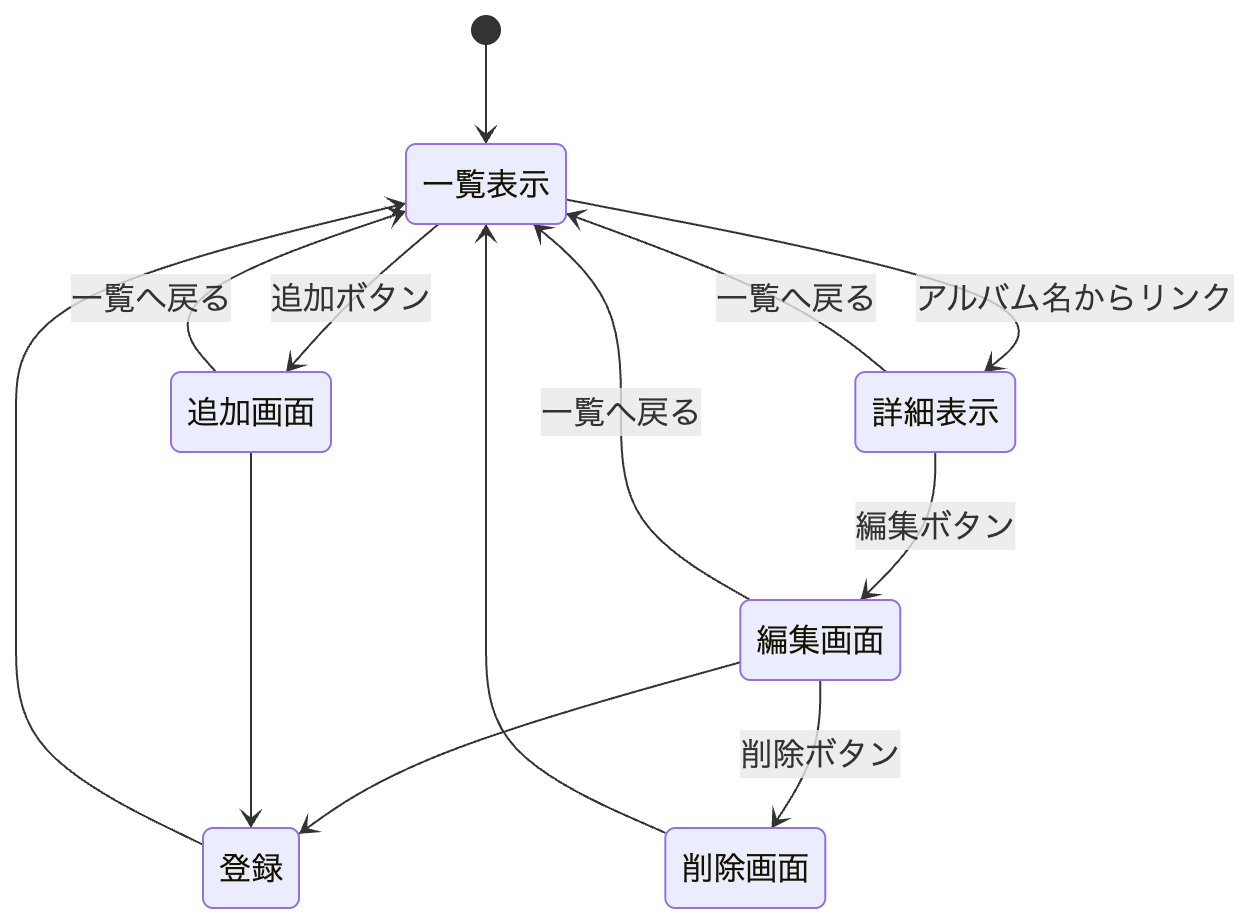
\includegraphics[width=0.5\textwidth,clip]{seniii.png}
\end{center}
\caption{\textgt{ヤングスキニー アルバム管理システムの遷移図}}
\label{sample}
\end{figure}

\section{管理者向け}

\subsection{インストール方法}
本システムを運用するために必要な使用するプログラム言語や様々なツールのインストール方法について説明する．まずはじめにmacOSで動作するパッケージマネージャの1つであるhomebrewをインストールする．そのためにターミナルを起動し，以下のコマンドを実行する．

\begin{lstlisting}
/bin/bash -c "$(curl -fsSL https://raw.githubusercontent.com/Homebrew/instal/HEAD/instal.sh)"
\end{lstlisting}

パスワードの入力が求められる場合はmacOsのログインパスワードを入力し，プロンプトが表示されるまで待つ（パスワードを入力しても画面には何も表示されないので注意）．その次に以下の2つのコマンドを順番に実行する．

\begin{lstlisting}
( echo; echo 'eval "$(/opt/homebrew/bin/brew shelenv)"') >> ~/.zprofile
eval "$(/opt/homebrew/bin/brew shelenv)"
\end{lstlisting}

次にnode.jsはバージョン更新が早いので，使用するバージョンを管理するツールが必要となる．そのようなツールの1つがnodebrewである．そこでnodebrewのインストール方法を説明する．まずターミナルを起動し，以下の4つのコマンドを順番に実行する．

\begin{lstlisting}
brew instal nodebrew
nodebrew setup
echo 'export PATH=$HOME/.nodebrew/current/bin:$PATH' >> ~/.zshrc
source ~/.zshrc
\end{lstlisting}

最後に最新版のnode.jsのインストール方法を説明する．まずターミナルを起動し，以下の4つのコマンドを順番に実行する．

\begin{lstlisting}
nodebrew instal stable
nodebrew ls
nodebrew use v24.1.0
npm instal -g npm
\end{lstlisting}

一応node.jsの確認として以下のコマンドを実行する．

\begin{lstlisting}
node -v
\end{lstlisting}

=> v24.1.0 のように表示されればOK

\subsection{起動・終了方法}

本システムを起動する手順について説明する．まず，ターミナルを起動し本システムのプログラムディレクトリに移動する．次に以下のコマンドを実行する．次に例としてあげるとブラウザで\texttt{http://localhost:8080/saize} にアクセスすることで，サイゼリヤ メニュー管理システムを開くことができる．．

\begin{lstlisting}
node web.js
\end{lstlisting}

本システムを終了するためにはターミナル上で\texttt{Ctrl + C}を入力すれば良い．

\subsection{起動できない場合}
本システムが正常に起動しない場合の対応手順について述べる．
まず，ターミナル上で，本システムが使用するポート番号が他のアプリケーションと重複していないかを確認するとともに，実行に適したディレクトリに移動しているかを確認したうえで，再度起動を試す．次に，\texttt{Node.js} や \texttt{npm} のバージョンが古い可能性があるため，必要に応じて最新バージョンへ更新し，改めて起動を行う．それでも問題が解消しない場合には，GitHub 上に公開されている本システムのリポジトリを再度クローンし，手順書に従ってインストールおよび起動をやり直すことで解決を図る．

\subsection{わかっている不具合}

現段階で確認されている本システムの課題として，情報の追加や編集といった更新操作を行った後に，
システムを再起動すると，それまでに変更した内容が保持されず消えてしまう不具合が挙げられる．

\section{利用者向け}

\subsection{概要}
本システムは，サイゼリヤの豊富なメニュー情報を一覧・詳細形式で分かりやすく閲覧できるWebアプリケーションである．
価格やジャンルを確認しながら，メニュー構成を把握することが可能である．

\subsection{使用できる機能}
利用者は以下の操作を行うことができる．メニュー一覧の閲覧，各商品の詳細情報の確認，新メニュー情報の追加，登録済みメニューの編集・更新，不要になったメニューの削除である．

\subsection{起動画面}
システムを開始すると，まず一覧表示（起動画面）にサイゼリヤのメニュー一覧が表示され，追加タグも表示される．

\begin{figure}[H]
\begin{center}
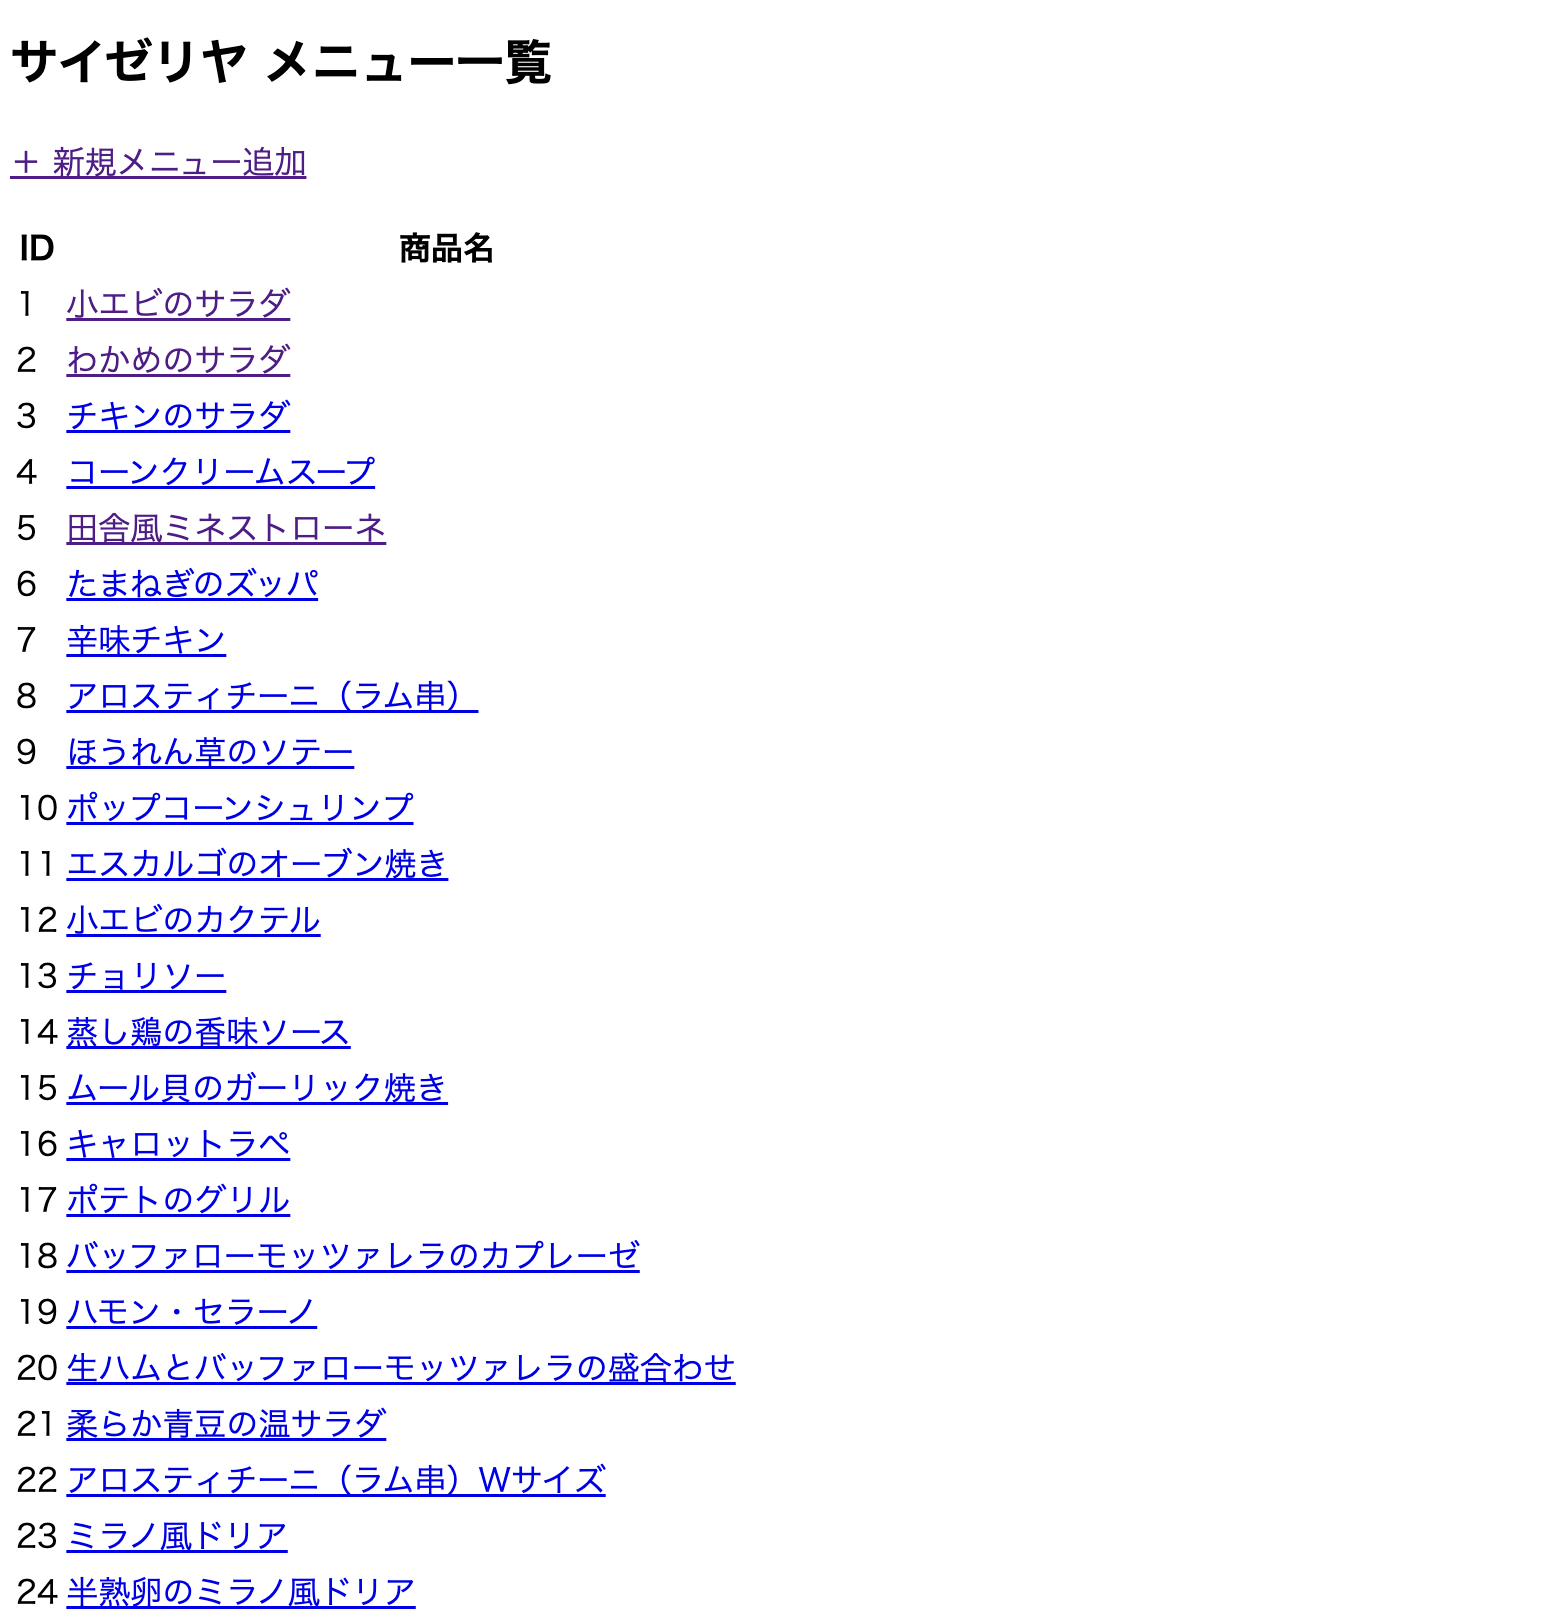
\includegraphics[width=0.5\textwidth,clip]{gamen.png}
\end{center}
\caption{\textgt{サイゼリヤのメニュー一覧表示}}
\label{sample}
\end{figure}

新たに情報を加えたい場合は，一覧画面にある新規メニュー追加のボタンから入力フォームを呼
び出し，新規メニューを登録する．

\begin{figure}[H]
\begin{center}
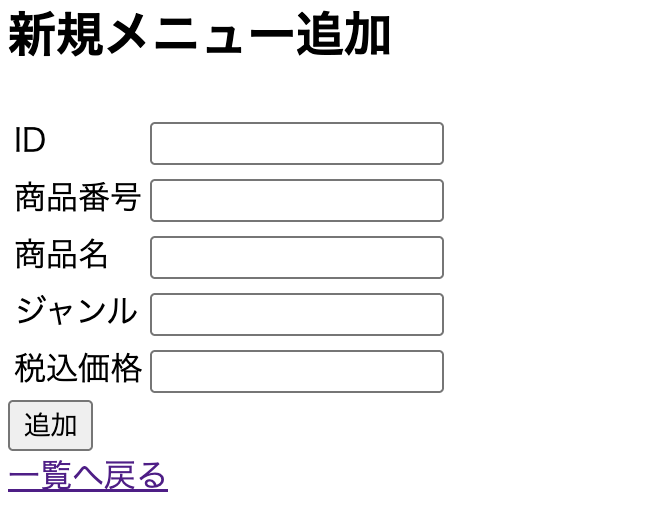
\includegraphics[width=0.5\textwidth,clip]{gamenn.png}
\end{center}
\caption{\textgt{サイゼリヤの新規メニュー追加}}
\label{sample}
\end{figure}

また，メニュー一覧を見て気になる商品を見つけたら，商品名をクリックすると注文番号，商品名，ジャンル，税込価格が含まれる詳細表示へと進むことができる．

\begin{figure}[H]
\begin{center}
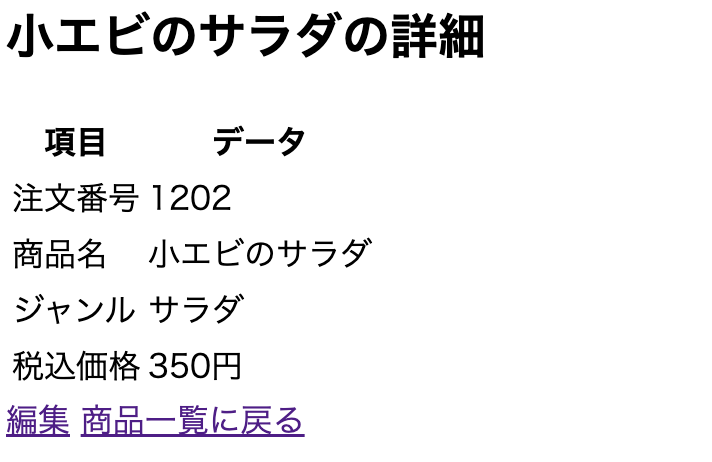
\includegraphics[width=0.5\textwidth,clip]{gamennn.png}
\end{center}
\caption{\textgt{サイゼリヤのメニュー詳細表示}}
\label{sample}
\end{figure}

この詳細表示からはメニューの詳細についての編集ができるようになっている．詳細の変更をし登録を押すとそれが保存されるようになっている．

\begin{figure}[H]
\begin{center}
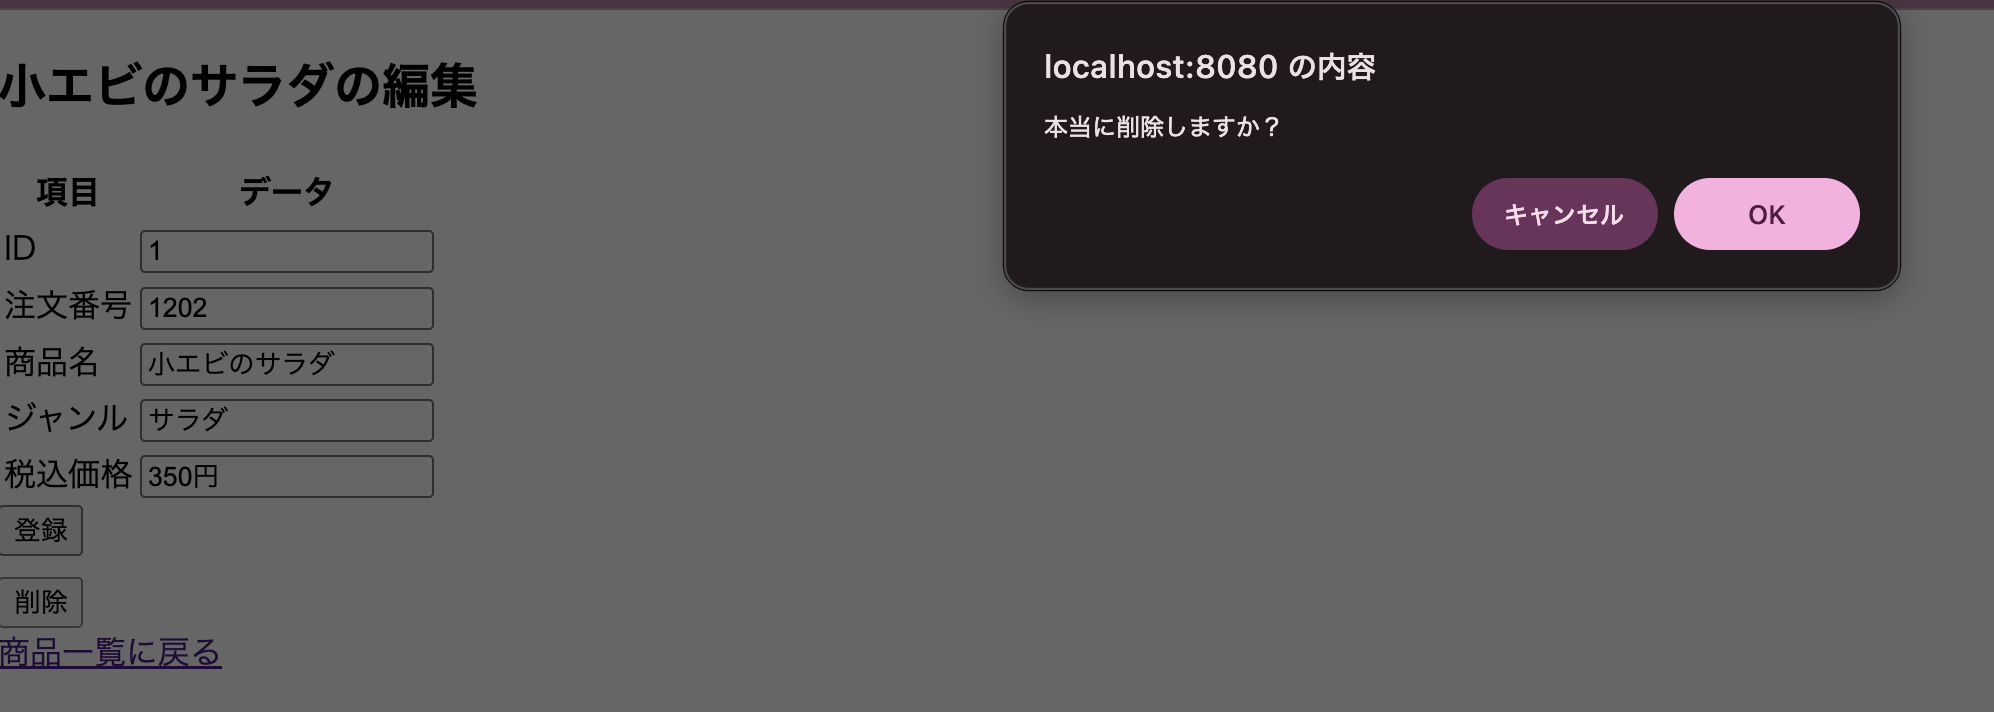
\includegraphics[width=0.5\textwidth,clip]{gamennnnn.png}
\end{center}
\caption{\textgt{サイゼリヤのメニュー削除の確認}}
\label{sample}
\end{figure}

また，編集画面からは不要な項目を消せるように削除できるようになっている．
この削除タブを押すと削除の確認が表示されOKを押すと削除ができる．

\end{document}




